\begin{name}
	{\tenchude}
	{TOÁN 12}
	{LỚP TOÁN THẦY PHÁT}
	{Thời gian: 90 phút - Không kể thời gian phát đề}
\end{name}
\Opensolutionfile{ansbook}[ans/ansbookDe4]
\TN
\Opensolutionfile{ans}[ans/ansDe4-TN1]
\begin{ex}%[2D4N1-1]
Cho hai hàm số $f(x)$, $g(x)$ là hàm số liên tục, có $F(x)$, $G(x)$ lần lượt là nguyên hàm của $f(x)$, $g(x)$. Xét các mệnh đề sau.
\begin{itemize}
\item[(i)] $F(x)+G(x)$ là một nguyên hàm của $f(x)+g(x)$.
\item[(ii)] $k\cdot F(x)$ là một nguyên hàm của $k\cdot f(x)$ với $k\in\mathbb{R}$.
\item[(iii)] $F(x)\cdot G(x)$ là một nguyên hàm của $f(x)\cdot g(x)$.
\end{itemize}
Các mệnh đề đúng là
\choice
{(ii) và (iii)}
{(i), (ii) và (iii)}
{(i) và (iii)}
{\True (i)}
\loigiai{
Theo tính chất của nguyên hàm, khẳng định (ii) sai khi $ k=0$, khẳng định (iii) sai.}
\end{ex}

\begin{ex}%[2D4N1-2]
Họ nguyên hàm của hàm số $y=x^2-3x+\dfrac{1}{x}$ là
\choice
{$\dfrac{x^3}{3}-\dfrac{3x^2}{2}-\ln\left|x\right|+C$}
{$\dfrac{x^3}{3}-\dfrac{3x^2}{2}+\ln x+C$}
{\True $\dfrac{x^3}{3}-\dfrac{3x^2}{2}+\ln\left|x\right|+C$}
{$\dfrac{x^3}{3}-\dfrac{3x^2}{2}+\dfrac{1}{x^2}+C$}
\loigiai{
Ta có
$\displaystyle\int \left(x^2-3x+\dfrac{1}{x}\right) \mathrm{\,d}x=\dfrac{x^3}{3}-\dfrac{3x^2}{2}+\ln\left|x\right|+C$.

}
\end{ex}

\begin{ex}%[2D4N2-1]Biên soạn:Phùng Hoàng Em Phản biện:Nguyễn Đắc Kiên
Cho hàm số $f(x)$ liên tục trên $\mathbb{R}$ và $a$ là số thực dương. Khẳng định nào sau đây là khẳng định đúng?
\choice
{$\displaystyle\int\limits_a^a f(x) \mathrm{\,d}x=1$}
{$\displaystyle\int\limits_a^af(x) \mathrm{\,d}x=a^2$}
{\True $\displaystyle\int\limits_a^af(x) \mathrm{\,d}x=0$}
{$\displaystyle\int\limits_a^a f(x) \mathrm{\,d}x=2a$}
\loigiai{
Gọi $F(x)$ là một nguyên hàm của $f(x)$.
Ta có $\displaystyle\int\limits_a^af(x) \mathrm{\,d}x=F(x)\Bigg|_a^a=F(a)-F(a)=0$.
}
\end{ex}

\begin{ex}%[2H5N1-1]%[Dự án Khối 12- Ex-TF-TLN-2024]%[VU Ngoc Hao]
\immini{
Cho hình hộp chữ nhật $ABCD.A'B'C'D'$. Bốn véc-tơ pháp tuyến  của mặt phẳng $\left(AA'B'B\right)$ là
\choice
{$\overrightarrow{AD}$, $\overrightarrow{A'D'}$, $ \overrightarrow{BD}$, $\overrightarrow{B'C'}$}
{$\overrightarrow{AD}$, $\overrightarrow{A'D'}$, $ \overrightarrow{BC}$, $\overrightarrow{BC'}$}
{$\overrightarrow{AC}$, $\overrightarrow{A'D'}$, $ \overrightarrow{BC}$, $\overrightarrow{B'C'}$}
{\True  $\overrightarrow{AD}$, $\overrightarrow{A'D'}$, $ \overrightarrow{BC}$, $\overrightarrow{B'C'}$}
}
{
\begin{tikzpicture}[scale=0.5, font=\footnotesize,line join=round, line cap=round, >=stealth]
\coordinate (A) at (0,0);
\coordinate (B) at (-2,-1.5);
\coordinate (D) at (5,0);
\coordinate (C) at ($(B)+(D)-(A)$);
\foreach \i in {A,B,C,D}{\coordinate (\i') at ($(\i)+(0,4)$);}
\draw (A')--(B')--(C')--(D')--cycle;
\draw (B)--(B') (C)--(C') (D)--(D')  (B)--(C)--(D);
\draw[dashed,thin](B)--(A)--(A') (A)--(D);
\foreach \i/\g in {A'/90,B'/90,C'/90,D'/90,A/-90,B/-90,C/-90,D/-90}{\draw[fill=black](\i) circle (1pt) ($(\i)+(\g:5mm)$) node[scale=1]{$\i$};}
\end{tikzpicture}
}
\loigiai{
Bốn véc-tơ pháp tuyến của mặt phẳng $\left(AA'B'B\right)$ là  $\overrightarrow{AD}$, $\overrightarrow{A'D'}$, $ \overrightarrow{BC}$, $\overrightarrow{B'C'}$.
}
\end{ex}

\begin{ex}%[Mức độ 1]%[BG-12-New-4in1, Hiệp Hà]%[2H5N1-2]
Cho $(\alpha)$ vuông góc với giá của $\vec{a}=(2;-1;3)$. Vectơ nào dưới đây là vectơ pháp tuyến của $(\alpha)$?
\choice
{$\vec{n_1}=(-2;1;3)$}
{\True $\vec{n_2}=(-2;1;-3)$}
{$\vec{n_3}=(4;2;6)$}
{$\vec{n_4}=(4;-2;-6)$}
\loigiai{
$(\alpha)$ vuông góc với giá của $\vec{a}=(2;-1;3)$ nên $\vec{a}$ là một vectơ pháp tuyến của $(\alpha)$.\\
Do đó $\vec{n_2}=-\vec{a}$ cũng là một vectơ pháp tuyến của $(\alpha)$.
}
\end{ex}

\begin{ex}%[2H5N2-1]%[Dự án EX-TF-TLN lần 3 - Nguyễn Thắng]
Trong không gian $Oxyz$, cho đường thẳng $\Delta$ đi qua điểm $M(x_0;y_0;z_0)$ và có véc-tơ chỉ phương $\vec{u}=(a;b;c)$ và $abc\ne 0$. Khi đó hệ phương trình nào sau đây là phương trình chính tắc của đường thẳng $\Delta$?
\choice
{$\dfrac{x-x_0}{a}=\dfrac{y+y_0}{b}=\dfrac{z+z_0}{c}$}
{$\dfrac{x+x_0}{a}=\dfrac{y+y_0}{b}=\dfrac{z+z_0}{c}$}
{$\dfrac{x+x_0}{a}=\dfrac{y+y_0}{b}=\dfrac{z-z_0}{c}$}
{\True $\dfrac{x-x_0}{a}=\dfrac{y-y_0}{b}=\dfrac{z-z_0}{c}$}
\loigiai{

}
\end{ex}

\begin{ex}%[2H5N2-2]%[Dự án 2025 - Đề cấu trúc mới của Bộ theo [Thành Đức Trung]
Trong không gian $Oxyz$, cho mặt phẳng $(P)\colon x-2y-3z-2=0$. Đường thẳng $d$ vuông góc với mặt phẳng $(P)$ có một véc-tơ chỉ phương là
\choice
{$\overrightarrow{u}_{1}=(1;-2;-2)$}
{\True $\overrightarrow{u}_{2}=(1;-2;-3)$}
{$\overrightarrow{u}_{4}=(1;2;3)$}
{$\overrightarrow{u}_{3}=(1;-3;-2)$}
\loigiai
{
Ta có $(P)\colon x-2y-3z-2=0$, suy ra một véc-tơ pháp tuyến của $(P)$ là $\overrightarrow{u}_{2}=(1;-2;-3)$.
}
\end{ex}

\begin{ex}%[2H5N3-2]
Trong không gian $Oxyz$, cho mặt cầu $(S)\colon x^2+(y-4)^2+(z-1)^2=25$. Tọa độ tâm $I$ và bán kính $R$ của mặt cầu $(S)$ là
\choice
{$I(0;-4;-1)$, $R=25$}
{$I(0;-4;-1)$, $R=5$}
{$I(0;4;1)$, $R=25$}
{\True $I(0;4;1)$, $R=5$}
\loigiai{
Mặt cầu $(S)$ có tâm $I(0;4;1)$ và bán kính $R=5$.
}
\end{ex}

\begin{ex}%[12-PTMH-1-2025]%[Võ Thị Thùy Trang]%[2D6N1-1]
Cho hai biến cố $A$ và $B$ bất kì, với $\mathrm{P}(B)>0$. Công thức tính xác suất nào sau đây là đúng?
\choice
{$\mathrm{P}(A\mid B)= \dfrac{\mathrm{P}(A)}{\mathrm{P}(B)}$}
{\True $\mathrm{P}(A\mid B)= \dfrac{\mathrm{P}(AB)}{\mathrm{P}(B)}$}
{$\mathrm{P}(A\mid B)= \dfrac{\mathrm{P}(AB)}{\mathrm{P}(A)}$}
{$\mathrm{P}(A\mid B)= \dfrac{\mathrm{P}(B)}{\mathrm{P}(A)}$}
\loigiai
{
Theo tính chất, công thức đúng là $\mathrm{P}(A\mid B)= \dfrac{\mathrm{P}(AB)}{\mathrm{P}(B)}$.
}
\end{ex}

\begin{ex}%[2D6N2-1]%[Lê Công Trường]
Giả sử tỉ lệ người dân của tỉnh Khánh Hòa nghiện thuốc lá là $\mathrm{P}(A)$; tỉ lệ người bị bệnh phổi
trong số người nghiện thuốc lá là $\mathrm{P}(B)$, trong số người không nghiện thuốc lá là $\mathrm{P}(B\mid \overline{A})$. Hỏi khi ta gặp ngẫu nhiên một người dân của tỉnh Khánh Hòa thì khả năng mà đó bị bệnh phổi là
\choice
{$\mathrm{P}(A)=\mathrm{P}(B)\cdot\mathrm{P}(A\mid B)+\mathrm{P}(\overline{B})\cdot\mathrm{P}(A\mid \overline{B})$}
{$\mathrm{P}(A)=\mathrm{P}(A)\cdot\mathrm{P}(A\mid B)+\mathrm{P}(\overline{A})\cdot\mathrm{P}(A\mid \overline{B})$}
{\True $\mathrm{P}(B)=\mathrm{P}(A)\cdot\mathrm{P}(B\mid A)+\mathrm{P}(\overline{A})\cdot\mathrm{P}(B\mid \overline{A})$}
{$\mathrm{P}(A\mid B)=\dfrac{\mathrm{P}(A)\cdot\mathrm{P}(B\mid A)}{\mathrm{P}(B)}$}
\loigiai{Khi ta gặp ngẫu nhiên một người dân của tỉnh Khánh Hòa thì khả năng mà đó bị bệnh phổi là \[\mathrm{P}(B)=\mathrm{P}(A)\cdot\mathrm{P}(B\mid A)+\mathrm{P}(\overline{A})\cdot\mathrm{P}(B\mid \overline{A}).\]}
\end{ex}

\begin{ex}%[2D6N2-3]%[Dự án EX-TF-TLN lần 4 - Quan Ón]
Cho hai biến cố $A$, $B$ sao cho $\mathrm{P}(A) = 0{,}6$; $\mathrm{P}(B) = 0{,}4$ ; $\mathrm{P}(B\mid A) = 0{,}2$. Khi đó, $\mathrm{P}(A\mid B)$ bằng
\choice
{$0{,}11$}
{$0{,}57$}
{$0{,}83$}
{\True $0{,}30$}
\loigiai{
Áp dụng công thức Bayes, ta có $\mathrm{P}(A\mid B) = \dfrac{\mathrm{P}(A)\cdot\mathrm{P}(B\mid A)}{\mathrm{P}(B)} = \dfrac{0{,}6\cdot 0{,}2}{0{,}4} = 0{,}3$.
}
\end{ex}

\begin{ex}%[2H5N3-3]
Trong không gian $Oxyz$, phương trình mặt cầu tâm $I(-1;2;0)$ và bán kính bằng $2$ là
\choice
{$(x+1)^{2}+(y-2)^{2}+z^{2}=4$}
{$(x-1)^{2}+(y+2)^{2}+z^{2}=2$}
{$(x+1)^{2}+(y-2)^{2}+z^{2}=2$}
{\True $(x-1)^{2}+(y+2)^{2}+z^{2}=4$}
\loigiai{
Phương trình mặt cầu tâm $I(-1;2-0)$ và bán kính bằng $2$ là \[(x-(-1))^{2}+(y-2)^{2}+z^{2}=4\] hay \[(x+1)^{2}+(y-2)^{2}+z^{2}=4.\]
}
\end{ex}
\Closesolutionfile{ans}

\TNTF
\Opensolutionfile{ans}[ans/ansDe4-TN2]
\begin{ex}%[2025-TLOT-2018,Trần Xuân Hòa]%[2D4H2-2]
Cho hàm số $f(x)=x(x^2+3)$. Xét $I=\displaystyle\int\limits_{-1}^1|f(x)|\mathrm{\; d}x$.
\choiceTF
{\True Đặt $I_1=\displaystyle\int\limits_{0}^1|f(x)|\mathrm{\; d}x$ và $I_2=\displaystyle\int\limits_{-1}^0|f(x)|\mathrm{\; d}x$. Khi đó $I_1=I_2$}
{Giá trị $I=0$}
{\True Số thực dương $m$ để $\displaystyle\int\limits_0^m|f(x)|\mathrm{\;d}x=4$ bằng $\sqrt{2}$}
{Số thực $a$ để $\displaystyle\int\limits_0^1x(x^2+3-a\sqrt{x})\mathrm{\; d}x=0$ bằng $4$}
\loigiai{
\begin{itemchoice}
\itemch Đúng.
\begin{itemize}
\item Ta có $I_1=\displaystyle\int\limits_0^1(x^3+3x)\mathrm{\; d}x=\left(\dfrac{x^4}{4}+\dfrac{3x^2}{2}\right)\bigg |_0^1=\dfrac{7}{4}$.
\item Ta có $I_2=\displaystyle\int\limits_{-1}^0(-x^3-3x)\mathrm{\; d}x=\left(-\dfrac{x^4}{4}-\dfrac{3x^2}{2}\right)\bigg |_{-1}^0=\dfrac{7}{4}$.
\end{itemize}
Do đó $I_1=I_2$.
\itemch Sai. Ta có $I=\displaystyle\int\limits_{-1}^0|f(x)|\mathrm{\; d}x+\displaystyle\int\limits_{0}^1|f(x)|\mathrm{\; d}x=I_1+I_2=\dfrac{7}{4}+\dfrac{7}{4}=\dfrac{7}{2}$.
\itemch Đúng. Ta có
\begin{eqnarray*}
&&\displaystyle\int\limits_0^m|f(x)|\mathrm{\;d}x=4\\
&\Leftrightarrow&\displaystyle\int\limits_0^{m}(x^3+3x)\mathrm{\;d}x=4\\
&\Leftrightarrow&\left(\dfrac{x^4}{4}+\dfrac{3x^2}{2}\right)\bigg |_0^m=4\\
&\Leftrightarrow&\dfrac{m^4}{4}+\dfrac{3m^2}{2}-4=0\\
&\Leftrightarrow&\hoac{&m=\sqrt{2}\\&m=-\sqrt{2} \text{ ( loại )}.}
\end{eqnarray*}
Vậy $m=\sqrt{2}$ thỏa mãn.
\itemch Sai. Ta có
\begin{eqnarray*}
&&\displaystyle\int\limits_0^1x(x^2+3-a\sqrt{x})\mathrm{\; d}x=0\\
&\Leftrightarrow&\displaystyle\int\limits_0^1\left(x^3+3x-ax^{\tfrac{3}{2}}\right)\mathrm{\; d}x=0\\
&\Leftrightarrow&\left(\dfrac{1}{4}x^4+\dfrac{3}{2}x^2-\dfrac{2a}{5}x^{\tfrac{5}{2}}\right)\bigg|_0^1=0\\
&\Leftrightarrow&\dfrac{7}{4}-\dfrac{2a}{5}=0\\
&\Leftrightarrow&a=\dfrac{35}{8}.
\end{eqnarray*}
\end{itemchoice}
}
\end{ex}
\begin{ex}%[2H5H1-4]
	Trong không gian $Oxyz$, cho mặt phẳng $(P)$ đi qua $A(3;-2;5)$ và có vectơ pháp tuyến $\vec{n}=(4;-3;2)$ và mặt phẳng $(R)\colon x+2y-z+6=0$.
	\choiceTF
	{Phương trình mặt phẳng $(P)$ là $3x-2y+5z-28=0$}
	{\True $(P)$ vuông góc với mặt phẳng $(R)$}
	{Mặt phẳng $(P)$ cắt mặt phẳng $(R)$ theo giao tuyến là đường thẳng $d\colon \dfrac{x-3}{4}=\dfrac{y+2}{-3}=\dfrac{z-5}{2}$}
	{\True Mặt cầu tâm $A(3;-2;5)$ và bán kính $R=2$ cắt mặt phẳng $(R)$ theo giao tuyến là đường tròn có bán kính bằng $2$}
	\loigiai{
	\begin{itemchoice}
	\itemch Sai. Phương trình mặt phẳng $(P)$ đi qua $A(3;-2;5)$ có một vectơ pháp tuyến $\vec{n}_{(P)}=(4;-3;2)$ có dạng $4(x-3)-3(y+2)+2(z-5)=0$, hay $(P)\colon 4x-3y+2z-28=0$.
	\itemch Đúng. Vì với $\vec{n}_{(P)}=(4;-3;2)$ và $\vec{n}_{(R)}=(1;2;1)$ lần lượt là vectơ pháp tuyến của $(P)$ và $(R)$, ta thấy $\vec{n}\cdot \vec{n}_2=0$ nên $(P)\perp (R)$.
	
	\end{itemchoice}
	}
	\end{ex}
\Closesolutionfile{ans}

\TNSA
\Opensolutionfile{ans}[ans/ansDe4-TN3]
\begin{ex}%[2D4H1-4]
Hàm số $f(x)$ có đạo hàm liên tục trên $\mathbb{R}$ và $f'(x)=2^x+3^x$, $\forall x$; $f(0)=\dfrac{1}{\ln3}$. Tính giá trị của $f(1)$. (Làm tròn đến số thập phân thứ hai)
\shortans{$4{,}17$}
\loigiai{
Hàm số $f(x)=\displaystyle \int (2^x+3^x)\mathrm{\,d}x= \displaystyle \int 2^x \mathrm{\,d}x+\displaystyle \int 3^x \mathrm{\,d}x=\dfrac{2^x}{\ln2}+\dfrac{3^x}{\ln3}+C$.\\
$f(x)=\dfrac{2^x}{\ln2}+\dfrac{3^x}{\ln3}+C$.\\
Do $f(0)=\dfrac{1}{\ln3} \Leftrightarrow \dfrac{1}{\ln3}=\dfrac{1}{\ln2}+\dfrac{1}{\ln3}+C\Leftrightarrow C=-\dfrac{1}{\ln2}$\\
Suy ra $f(x)=\dfrac{2^x}{\ln2}+\dfrac{3^x}{\ln3}-\dfrac{1}{\ln2}$.\\
Vậy $f(1)=4{,}17$.
}
\end{ex}

\begin{ex}%[2D4V2-6]
Một vật chuyển động trong $6$ giờ với vận tốc $v$ (km/h) phụ thuộc vào thời gian $t$ (h) có đồ thị như hình bên dưới. Trong khoảng thời gian $2$ giờ từ khi bắt đầu chuyển động, đồ thị là một phần đường Parabol có đỉnh $I\left(3;9\right)$ và có trục đối xứng song song với trục tung. Khoảng thời gian còn lại, đồ thị vận tốc là một đường thẳng có hệ số góc bằng $\dfrac{1}{4}$. Tính quảng đường $s$ mà vật di chuyển được trong $6$ giờ? (đơn vị tính bằng km, làm tròn đến chữ số thập phân thứ nhất).
\begin{center}
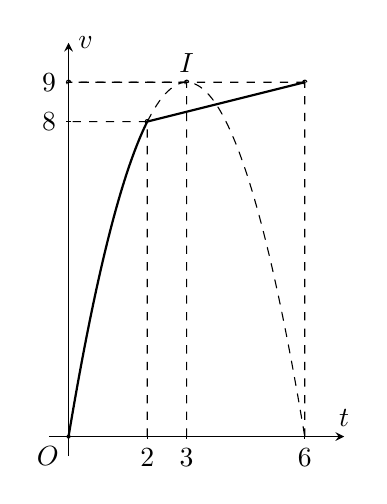
\begin{tikzpicture}[>=stealth,scale=0.5]
% Vẽ 2 trục, điền các số lên trục
\draw[->] (-0.5,0)--(0,0) node[below left]{$O$}--(7,0) node[above]{$t$}; %định dạng trục Ox
\foreach \x in {2,3,6}
\draw[shift={(\x,0)},color=black] (0pt,2pt)--(0pt,-2pt)
node[below] { $\x$};
\draw[->,color=black] (0,-0.5)--(0,10) node[right]{$v$};  %định dạng trục Oy
\foreach \y in {8,9}
\draw[shift={(0,\y)},color=black] (2pt,0pt) -- (-2pt,0pt)
node[left] {$\y$};
\clip(-1,-1) rectangle (7,10); %vùng đồ thị
%\draw[gray!50,thin,opacity=.5] (-1,-1) grid (4,10); %ô vuông
%Vẽ đồ thị
\draw[smooth,samples=100,domain=0:2,font=\footnotesize, line join=round, line cap=round, thick]
plot(\x,{(-1)*(\x)^2+6*(\x)});
\draw[smooth,domain=2:6, line join=round, line cap=round,dashed]
plot(\x,{(-1)*(\x)^2+6*(\x)});
\draw[smooth,samples=100,domain=2:6,font=\footnotesize, line join=round, line cap=round, thick]
plot(\x,{(1/4)*(\x)+15/2});
% Vẽ thêm mấy cái râu ria
\draw[dashed] (3,0)--(3,9) circle(1.5pt) node[above]{$I$}--(0,9) circle(1.5pt);
\draw[dashed] (2,0)--(2,8) circle(1.5pt) --(0,8);
\draw[dashed] (6,0)--(6,9) circle(1.5pt) --(0,9);
%Vẽ dấu chấm tròn
\fill (0cm,0cm) circle (1.5pt);
\end{tikzpicture}
\end{center}
\shortans{$43{,}3$}
\loigiai{
Vì Parabol đi qua $O\left(0;0\right)$ và có tọa độ đỉnh $I\left(3;9\right)$ nên thiết lập được phương trình Parabol là $\left(P\right) \colon y = v\left(t\right) = -t^2+6t$; $\forall t \in \left[0;2\right]$.\\
Sau $2$ giờ đầu thì hàm vận tốc có dạng là hàm bậc nhất $y = \dfrac{1}{4}t + m$, dựa trên đồ thị ta thấy đi qua điểm có tọa độ $\left(6;9\right)$ nên thế vào hàm số và tìm được $m = \dfrac{15}{2}$.\\
Nên hàm vận tốc từ giờ thứ $2$ đến giờ thứ $6$ là: $y = \dfrac{1}{4}t + \dfrac{15}{2},\forall t \in \left[2;6\right]$.\\
Quảng đường vật đi được bằng tổng đoạn đường $2$ giờ đầu và đoạn đường $4$ giờ sau.
\[S = S_1 +S_2 = \displaystyle\int\limits_0^2 \left(-t^2+6t\right) \mathrm{\,d}t + \displaystyle\int\limits_2^6 \left(\dfrac{1}{4}t+\dfrac{15}{2} \right) \mathrm{\,d}t = \dfrac{130}{3} \approx 43{,}3 \left(\text{km}\right).\]
}
\end{ex}

\begin{ex}%[Nguyễn Tuấn, dự án TLDT-2]%[2H5V2-8]
	Trong không gian $Oxyz$, hai máy bay cùng xuất phát từ hai phi trường, trên màn hình rađa của trạm điều khiển (với đơn vị trên ba trục chính theo đơn vị km), sau khi xuất phát $ t$ giờ $(t\ge 0)$, vị trí của máy bay số một được xác định bởi công thức $\heva{&x=20+2t \\ &y=20+t \\ &z=-10-t }$, vị trí máy bay số hai có tọa độ là $(30+t';20+t';-10-t')$. Hỏi nếu hai máy bay không thay đổi đường bay thì sau bao lâu thì hai máy bay có thể va chạm nhau?
	\shortans{10}
	\loigiai{
		Giả sử đường bay của máy bay số 1 là $(\Delta_1)\colon \heva{&x=20+2t \\ &y=20+t \\ &z=-10-t }$ có $\overrightarrow{u}_1=(2;1;-1)$ và đường bay của máy bay số 2 thỏa $(30+t';20+t';-10-t')\in (\Delta_2)\colon \heva{&x=30+t' \\ &y=20+t' \\ &z=-10-t' }$ có $\overrightarrow{u}_2=(1;1;-1)$.\\
		Kể từ thời điểm xuất phát, để hai may bay gần nhau nhất thì hai máy bay phải gần tọa độ giao điểm của $\Delta_1$ và $\Delta_2$.\\
	Ta có $\heva{&20+2t=30+t' \\ &20+t=20+t' \\ &-10-t=-10-t' }\Leftrightarrow \heva{&2t-t'=10 \\ &t-t'=0 \\ &t-t'=0 }\Leftrightarrow \heva{&t=10 \\ &t'=10.}$\\
	Vậy sau $10$ giờ thì hai máy bay có thể va chạm nhau.
	}
	\end{ex}

\begin{ex}%[2D6V1-3]
Trường Hạnh Phúc có $20$\% học sinh tham gia câu lạc bộ âm nhạc, trong số học sinh đó có $85$\% học sinh biết chơi đàn guitar. Ngoài ra, có $10$\% số học sinh không tham câu lạc bộ âm nhạc cũng biết chơi đàn guitar. Chọn ngẫu nhiên $1$ học sinh của trường. Giả sử học sinh đó biết chơi đàn guitar. Xác suất chọn được học sinh thuộc câu lạc bộ âm nhạc là bao nhiêu?

\shortans{0,68}
\loigiai
{
Gọi $A$ là biến cố \textquotedblleft Số học sinh thuộc câu lạc bộ âm nhạc\textquotedblright.\\
$B$ là biến cố \textquotedblleft Số học sinh không thuộc câu lạc bộ\textquotedblright.\\
Khi đó $\heva{&P(A) = 20\% = 0{,}2 &\Rightarrow& P(\overline{A}) = 1-0{,}2 = 0{,}8\\ &P(B|A) = 85\% = 0{,}85 &\Rightarrow& P(\overline{B}|A) = 1-0{,}85 = 0{,}15\\ &P(B|\overline{A}) = 10\% = 0{,}1 &\Rightarrow& P(\overline{B}|\overline{A}) = 1-0{,}1=0{,}9.}$
\begin{center}
\begin{tikzpicture}[>=stealth]
%Khung 1
\draw (-0,-1) rectangle (2.2,0);
\draw (1.1,-0.5) node{Gốc};
%Mui ten 1,2
\draw [->] (2.2,-0.5)--(3.8,1.6) node[pos=0.5,sloped,above]{$0{,}2$};
\draw [->] (2.2,-0.5)--(3.8,-2.6) node[pos=0.5,sloped,below]{\color{red}$0{,}8$};
%Khung 2.1
\draw (4.5,3.0) node{\textbf{Thuộc câu lạc bộ}};
\draw (3.8,1.1) rectangle (5.1,2.1);
\draw (8.9/2,1.6) node{$A$} ;
%Khung 2.2
\draw (3.8,-2.1) rectangle (5.1,-3.1);
\draw (8.9/2,-2.6) node{$\overline{A}$};
%Mui ten 3,4
\draw [->] (5.1,1.6)--(6.5,2.6) node[pos=0.5,sloped,above]{$0{,}85$};
\draw [->] (5.1,1.6)--(6.5,0.6) node[pos=0.5,sloped,below]{\color{red}$0{,}15$};
%Mui ten 5,6
\draw [->] (5.1,-2.6)--(6.5,-1.6) node[pos=0.5,sloped,above]{$0{,}1$};
\draw [->] (5.1,-2.6)--(6.5,-3.6) node[pos=0.5,sloped,below]{\color{red}$0{,}9$};
%Khung 3.1
\draw (6.5,2.2) rectangle (7.7,3.2);
\draw (7.1,5.4/2) node{$B$} ;
%Khung 3.2
\draw (6.7,3.7) node{\textbf{Biết chơi guitar}};
\draw (6.5,1.2) rectangle (7.7,0.2);
\draw (7.1,1.4/2) node{$\overline{B}$} ;
%Khung 3.3
\draw (6.5,-1.1) rectangle (7.7,-2.1);
\draw (7.1,-3.2/2) node{$B$} ;
%Khung 3.3
\draw (6.5,-2.9) rectangle (7.7,-3.9);
\draw (7.1,-3.4) node{$\overline{B}$} ;
%Kết quả
\draw (9.5,3.7) node{\textbf{Kết quả}};
\draw (9.5,2.7) node{$AB$};
\draw (9.5,0.7) node{$A \overline{B}$};
\draw (9.5,-1.6) node{$\overline{A}B$};
\draw (9.5,-3.4) node{$\overline{A}~\overline{B}$};
%Xác suất
\draw (12.5,3.7) node{\textbf{Xác suất}};
\draw (12.5,2.7) node{$0{,}17$};
\draw (12.5,0.7) node{$0{,}03$};
\draw (12.5,-1.6) node{$0{,}08$};
\draw (12.5,-3.4) node{$0{,}72$};
\end{tikzpicture}
\end{center}
Áp dụng công thức xác suất Bayes để tính xác chọn được học sinh thuộc câu lạc bộ âm nhạc
\[P(A|B) = \dfrac{P(A)\cdot P(B|A)}{P(A) \cdot P(B|A) + P(\overline{A}) \cdot P(B|\overline{A})} = \dfrac{0{,}2 \cdot 0{,}85}{0{,}2 \cdot 0{,}85 + 0{,}8\cdot 0{,}1} = 0{,}68.\]
}
\end{ex}
\TL
\begin{ex}%[2H5H2-3]%[Dự án EX-TF-TLN lần 3 - Nguyen Chín Em]
Trong không gian với hệ tọa độ $Oxyz$. Viết phương trình tham số của đường thẳng $d$ biết $d$ đi qua điểm $M(2; -3; 4)$, vuông góc với $d_1$ và $d_2: \dfrac{x + 1}{2} = \dfrac{y}{5} =\dfrac{z + 3}{3}$. Khi đó đường thẳng $d$ đi qua điểm $(x_0;y_0;-13)$. Tính $x_0^{2}+y_0^{2}$.
% \shortans{$125$}
\loigiai{
Ta có véc-tơ chỉ phương của $d_1$ là $\overrightarrow{u_1} = (-3; 1; 2)$ và véc-tơ chỉ phương của $d_2$ là $\overrightarrow{u_2} = (2; 5; 3)$.\\
Do $d \perp d_1$ và $d \perp d_2$ nên véc-tơ chỉ phương của $d$ là $\overrightarrow{u} =\left[\overrightarrow{u_1}, \overrightarrow{u_2}\right] = (-7; 13; -17)$.\\
Phương trình tham số của đường thẳng $d$ là $\heva{&x = 2 - 7t \\&y = -3 + 13t \\&z = 4 - 17t},(t\in\mathbb{R})$.\\
% Với $t=1$ đường thẳng $d$ đi qua điểm $(-5;10;-13)$, suy ra $x_0^{2}+y_0^{2}=125$.
}
\end{ex}

\begin{ex}%[12-PTMH-1-2025]%[Võ Thị Thùy Trang]%[2D6C2-4]
Ở một khu rừng nọ có $7$ chú lùn, trong đó có $4$ chú luôn nói thật, $3$ chú còn lại luôn tự nhận mình nói nhật nhưng xác suất để mỗi chú này nói thật là $0{,}5$. Bạn Tuyết gặp ngẫu nhiên một chú lùn. Gọi $A$ là biến cố \lq \lq Chú lùn đó luôn nói thật\rq \rq \, và $B$ là biến cố \lq \lq Chú lùn đó tự nhận mình luôn nói thật\rq \rq.
Biết rằng chú lùn mà bạn Tuyết gặp tự nhận mình là người luôn nói thật. Biết xác suất để chú lùn đó luôn nói thật có thể được biểu diễn dưới dạng $\dfrac{a}{b}$ sao cho $\dfrac{a}{b}$ là phân số tối giản. Tính $2a+b$.
% \shortans{$27$}
\loigiai{

Gọi $A$ là biến cố \lq \lq Chú lùn bạn Tuyết gặp luôn nói thật\rq \rq
\,và $B$ là biến cố \lq \lq Chú lùn đó luôn tự nhận mình nói thật\rq \rq.\\
Vì có $4$ chú lùn luôn nói thật nên xác suất để bạn Tuyết gặp chú lùn luôn nói thật là $\mathrm{P}(A)=\dfrac{4}{7}$ và gặp chú lùn tự nhận mình luôn nói thật là $\mathrm{P}(\overline{A})=\dfrac{3}{7}$.\\
Theo đề bài, ta có $\mathrm{P}(B\mid A)=1$, $\mathrm{P}(B\mid \overline{A})=0{,}5$.\\
Theo công thức xác suất toàn phần, ta có
\begin{align*}
\mathrm{P}(B) &=\mathrm{P}(B\mid A)\cdot\mathrm{P}(A)+\mathrm{P}(B\mid\overline{A})\cdot\mathrm{P}(\overline{A})\\
&=1 \cdot \dfrac{4}{7} + 0{,}5 \cdot \dfrac{3}{7}\\
&=\dfrac{11}{14}.
\end{align*}
Theo công thức Bayes, ta có
\[\mathrm{P}(A\mid B)=\dfrac{\mathrm{P}(B\mid A) \cdot \mathrm{P}(A)}{\mathrm{P}(B)}=\dfrac{1 \cdot \dfrac{4}{7}}{\dfrac{11}{14}}=\dfrac{8}{11}.\]
Vậy nếu chú lùn mà bạn Tuyết gặp tự nhận mình là người luôn nói thật, xác suất để chú lùn đó luôn nói thật là $\dfrac{8}{11}$.\\
Do đó $a=8$, $b=11$ nên $2a+b=2 \cdot 8+11=27$.
}
\end{ex}

\begin{ex}%[Mức độ ]giảng 12 New - 4in1, Đoàn Hùng]%[2H5V1-7]
	\immini
	{Trong không gian với hệ tọa độ $Oxyz$ (đơn vị trên mỗi trục toạ độ là km), một máy bay đang ở vị trí $A(3;-2{,}5; 0{,}5)$ và sẽ hạ cánh ở vị trí $B(3; 7{,}5; 0)$ trên đường băng (hình bên). Có một lớp mây được mô phỏng bởi một mặt phẳng $(\alpha)$ đi qua ba điểm $M(9;0;0)$, $N(0;-9;0)$, $P(0;0;0{,}9)$. Tính độ cao của máy bay khi máy bay xuyên qua đám mây để hạ cánh.}
	{\begin{tikzpicture}[line join = round, line cap = round,>=stealth,font=\footnotesize,scale=.5]
	\path
	(0,0) coordinate (O)
	(-9,0) coordinate (N)
	($(O)!1!40:(N)$) coordinate (M)
	(0,0.9) coordinate (P)
	($(O)!1.2!(M)$) coordinate (x)
	(-5,0.8) coordinate (A)
	(4,-1.5) coordinate (B)
	($(A)!2.1cm!(B)$) coordinate (C)
	(intersection of A--B and O--M) coordinate (B1)
	;
	\draw[line width=0.3mm,red] (A)--(C) (B1)--(B);
	\draw[line width=0.3mm,red,dashed] (C)--(B1);
	\draw[->,>=stealth,line width=0.3mm,blue] (0,0)--(x) node[right=0.2cm]{$x$};
	\draw[->,>=stealth,line width=0.3mm,blue] (-10,0)--(-9,0) (0,0) node[above right]{$O$}--(7,0) node[below]{$y$};
	\draw[line width=0.3mm,blue,dashed] (-9,0)--(0,0);
	\draw[->,>=stealth,line width=0.3mm,blue] (0,0)--(0,3) node[left]{$z$};
	\draw[line width=0.3mm,blue] (N)--(P)--(M) (N)--(M);
	\foreach \x/\gm in {N/90,P/140} \fill (\x) circle (1pt) ($(\x)+(\gm:5mm)$)node[blue]{$\x$};
	\filldraw[red] (N)node[below left,blue]{$-9$} (P)node[blue,above right]{$0{,}9$} (M)node[blue,right=0.1cm]{$9$}node[blue,left=0.1cm]{$M$} (C) circle (3pt) node[below=0.2cm,blue]{\scriptsize $C$} (A) circle (3pt)node[above left,red,blue]{$A$} (B)circle (3pt) node[below,blue]{$B$};
	\end{tikzpicture}}
	\shortans{$0{,}45$}
	\loigiai{
	Giả sử điểm $C\left(x_C;y_C;z_C\right)$ là vị trí mà máy bay xuyên qua đám mây để hạ cánh, suy ra $C\in (\alpha)$. Áp dụng phương trình mặt phẳng theo đoạn chắn, ta thấy mặt phẳng $(\alpha)$ có phương trình là
	\[\dfrac{x}{9}-\dfrac{y}{9}+\dfrac{z}{0{,}9}=1 \Leftrightarrow x-y+10z=9 \Rightarrow x_C-y_C+10z_C=9.\]
	Mặt khác, vì $\vec{AC}$, $\vec{AB}$ là hai véc-tơ cùng hướng nên tồn tại số thực $t>0$ sao cho $\vec{AC}=t\cdot \vec{AB}$.\\
	Do $\vv{AC}=\left(x_C-3;y_C+2{,}5;z_C-0{,}5\right)$; $\vv{AB}=\left(3-3;7{,}5+2{,}5;0-0{,}5\right)=\left(0;10;-0{,}5\right)$\\
	nên $\heva{&x_C-3=0t\\&y_C+2{,}5=10t\\&z_C-0{,}5=-0{,}5t} \Leftrightarrow \heva{&x_C=3\\&y_C=10t-2{,}5\\&z_C=-0{,}5t+0{,}5.}$\\
	Vì $C\in(\alpha)$ nên $3-(10 t-2{,}5)+10(-0{,}5 t+0{,}5)=9 \Leftrightarrow t=0{,}1$. Suy ra $C(3;-1{,}5;0{,}45)$.\\
	Vậy tại vị trí $C$, độ cao của máy bay là $0{,}45$ km.
	}
	\end{ex}
\Closesolutionfile{ans}

\Closesolutionfile{ansbook}

%
